
\section{\BookRecordIndex{T0023}Grothendieck--Knudsen 流形}\label{sec:D-4}

\noindent\textbf{嵌入的构造。}
本节构造一个自然的单射 $\overline{\mathcal M}_{0,n}\to(S^2)^N$，其像记为
$\overline M_{0,n}$。主要工具是黎曼球面 $S^2=\mathbb C\cup\{\infty\}$
上四点的\BookRecordIndex{T0185}交比
\[
  w(z_0,z_1,z_2,z_3)=
  \frac{(z_1-z_2)(z_3-z_0)}{(z_0-z_1)(z_2-z_3)}.
\]
其定义域是 $(S^2)^4$ 中至少有三点相等的集合 $\Delta_3$ 的补集；
有关性质列于 D.1 节。该定义可扩展到\BookRecordIndex{T0339}稳定曲线上的任意四个互异\BookRecordIndex{T0066}标记点
$\{i,j,k,\ell\}$：先用忘掉除 $z_i,z_j,z_k,z_\ell$ 之外所有点的映射
$\overline{\mathcal M}_{0,n}\to\overline{\mathcal M}_{0,4}$，再复合\BookRecordIndex{T0185}交比映射
$\overline{\mathcal M}_{0,4}\to S^2$。下面的引理给出它的显式公式。

\begin{lemma}\label{lem:D-4-1}
设 $\mathbf z=\bigl(\{z_{\alpha\beta}\}_{\alpha E\beta},
\{\alpha_i,z_i\}_{1\le i\le n}\bigr)\in SC_{0,n}$，
且 $i,j,k,\ell\in\{1,\ldots,n\}$ 两两互异。则：
\begin{enumerate}
\item[(i)] 存在 $\alpha\in T$，使
$(z_{\alpha i},z_{\alpha j},z_{\alpha k},z_{\alpha\ell})\notin\Delta_3$；
\item[(ii)] 若 $\alpha,\beta\in T$ 对应的两个四元组都不在 $\Delta_3$ 中，则
\[
  w(z_{\alpha i},z_{\alpha j},z_{\alpha k},z_{\alpha\ell})
  =w(z_{\beta i},z_{\beta j},z_{\beta k},z_{\beta\ell}).
\]
\end{enumerate}
\end{lemma}
\begin{proof}
断言 (i) 由注~\ref{rem:D-3-3} 得出：取 $\alpha=\alpha(i,j,k)$，则
$z_{\alpha i},z_{\alpha j},z_{\alpha k}$ 两两互异。
为证明 (ii)，先假设四点 $z_{\alpha i},z_{\alpha j},z_{\alpha k},
z_{\alpha\ell}$ 两两互异。此时 $\alpha$ 是满足 (i) 的唯一顶点。
事实上，若 $\beta\ne\alpha$，则存在 $\gamma\in T$，使
$\alpha E\gamma$ 且 $\beta\in T_{\alpha\gamma}$。四个顶点
$\alpha_i,\alpha_j,\alpha_k,\alpha_\ell$ 中至少三个位于
$T_{\gamma\alpha}$，从 $\beta$ 出发沿同一条边到达它们。
故 $z_{\beta i},z_{\beta j},z_{\beta k},z_{\beta\ell}$ 中相应三点重合。

若 $z_{\alpha i},z_{\alpha j},z_{\alpha k},z_{\alpha\ell}$
并非两两互异，则由假设至多两点重合，比如
$z_{\alpha\ell}=z_{\alpha k}$。由此
\[
  [\alpha_i,\alpha_j]\cap[\alpha_k,\alpha_\ell]=\varnothing,
  \qquad w(z_{\alpha i},z_{\alpha j},z_{\alpha k},z_{\alpha\ell})=\infty.
\]
设 $\beta\in T$ 是使相应四元组不在 $\Delta_3$ 中的另一顶点。
若 $\beta\notin[\alpha_i,\alpha_j]$，则 $z_{\beta i}=z_{\beta j}$；
若 $\beta\notin[\alpha_k,\alpha_\ell]$，则
$z_{\beta k}=z_{\beta\ell}$。两种情况必居其一，故
$w(z_{\beta i},z_{\beta j},z_{\beta k},z_{\beta\ell})=\infty$。
\end{proof}

因此，对每个互异的 $i,j,k,\ell\in\{1,\ldots,n\}$ 定义映射
$w_{ijk\ell}:\overline{\mathcal M}_{0,n}\to S^2$：对
$\mathbf z\in SC_{0,n}$ 取满足引理~\ref{lem:D-4-1} 的 $\alpha$，令
\begin{equation}\label{eq:D-4-1}
  w_{ijk\ell}(\mathbf z):=
  w(z_{\alpha i},z_{\alpha j},z_{\alpha k},z_{\alpha\ell})
  =\frac{(z_{\alpha j}-z_{\alpha k})(z_{\alpha\ell}-z_{\alpha i})}
  {(z_{\alpha i}-z_{\alpha j})(z_{\alpha k}-z_{\alpha\ell})}.
\end{equation}
引理说明此定义不依赖 $\alpha$；\BookRecordIndex{T0185}交比的 Möbius 不变性又说明右边
在定义~\ref{def:D-3-4} 的等价关系下不变。

置换 $i,j,k,\ell$ 的效果由\BookRecordIndex{T0185}交比的对称性质支配：
\begin{equation}\label{eq:D-4-2}
  w_{jik\ell}=w_{ij\ell k}=1-w_{ijk\ell},\qquad
  w_{ikj\ell}=\frac{w_{ijk\ell}}{w_{ijk\ell}-1}.
\end{equation}
见 D.1 节。\BookRecordIndex{T0185}交比的递推性质~\eqref{eq:D-1-3} 给出条件
\begin{equation}\label{eq:D-4-3}
  (1,\infty,w_{ijk\ell},w_{ijkm})\notin\Delta_3
  \quad\Longrightarrow\quad
  w_{jk\ell m}=\frac{w_{ijkm}-1}{w_{ijkm}-w_{ijk\ell}}
\end{equation}
对任意两两互异的 $i,j,k,\ell,m\in\{1,\ldots,n\}$ 成立。
令 $N:=n(n-1)(n-2)(n-3)$，并把 $(S^2)^N$ 的点写成元组
$w=\{w_{ijk\ell}\}_{1\le i,j,k,\ell\le n}$，仅取四指标互异者。
定义
\begin{equation}\label{eq:D-4-4}
  \overline M_{0,n}:=
  \bigl\{w=\{w_{ijk\ell}\}\in(S^2)^N\mid
  w\text{ 满足~\eqref{eq:D-4-2} 和~\eqref{eq:D-4-3}}\bigr\}.
\end{equation}
下一个定理是本附录的主要结果。

\begin{theorem}\label{thm:D-4-2}
\begin{enumerate}
\item[(i)] 若 $\mathbf z\in SC_{0,n}$，则式~\eqref{eq:D-4-1}
定义的元组 $w_{ijk\ell}=w_{ijk\ell}(\mathbf z)$ 满足
式~\eqref{eq:D-4-2} 与~\eqref{eq:D-4-3}，从而属于 $\overline M_{0,n}$。
\item[(ii)] 式~\eqref{eq:D-4-1} 定义的映射
$\overline{\mathcal M}_{0,n}\to\overline M_{0,n}$ 是双射。
\item[(iii)] $\overline M_{0,n}$ 是
$(S^2)^{n(n-1)(n-2)(n-3)}$ 的复子流形。
\end{enumerate}
\end{theorem}

\noindent\textbf{定理~\ref{thm:D-4-2}(i) 的证明。}
令 $\alpha=\alpha(i,j,k)\in T$ 为使
$z_{\alpha i},z_{\alpha j},z_{\alpha k}$ 两两互异的唯一顶点
（见注~\ref{rem:D-3-3}）。不妨设
$z_{\alpha i}=0,z_{\alpha j}=1,z_{\alpha k}=\infty$，
$z_{\alpha\ell}=w_{ijk\ell}$，$z_{\alpha m}=w_{ijkm}$。
于是按假设 $(z_{\alpha j},z_{\alpha k},z_{\alpha\ell},
z_{\alpha m})\notin\Delta_3$，故
\[
  w_{jk\ell m}=
  \frac{(z_{\alpha k}-z_{\alpha\ell})(z_{\alpha m}-z_{\alpha j})}
  {(z_{\alpha j}-z_{\alpha k})(z_{\alpha\ell}-z_{\alpha m})}
  =\frac{w_{ijkm}-1}{w_{ijkm}-w_{ijk\ell}}.
\]
这证明了定理~\ref{thm:D-4-2}(i)。\qed

\noindent\textbf{逆映射的构造。}
证明定理~\ref{thm:D-4-2}(ii) 的主要工具是 \BookRecordIndex{T0009}$w$-分割。
它使我们能把 $w\in\overline M_{0,n}$ 对应的树结构恢复为指标集
$\{1,\ldots,n\}$ 的\BookRecordIndex{T0124}分割网络。固定 $w\in\overline M_{0,n}$。
若一个 \BookRecordIndex{T0008}$n$-分割 $I\in\mathcal I_n$ 满足
\[
  i,i'\in I,\quad j,j'\notin I
  \quad\Longrightarrow\quad w_{ii'jj'}=\infty,
\]
则称 $I$ 为\emph{\BookRecordIndex{T0009}$w$-分割}（或 $(w,n)$-分割）。
其全体记为 $S(w)$。

\begin{lemma}\label{lem:D-4-3}
若 $w\in\overline M_{0,n}$，则 $S(w)$ 是一个 \BookRecordIndex{T0008}$n$-分割网络。
此外，下图交换：
\begin{equation}\label{eq:D-4-5}
  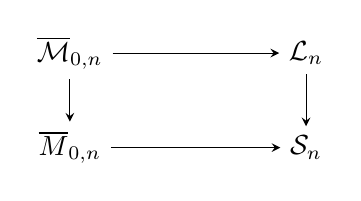
\begin{tikzpicture}[baseline=(current bounding box.center),>=stealth]
    \node (a) at (0,1.2) {$\overline{\mathcal M}_{0,n}$};
    \node (b) at (3,1.2) {$\mathcal L_n$};
    \node (c) at (0,0) {$\overline M_{0,n}$};
    \node (d) at (3,0) {$\mathcal S_n$};
    \draw[->] (a)--(b); \draw[->] (a)--(c);
    \draw[->] (b)--(d); \draw[->] (c)--(d);
  \end{tikzpicture}
\end{equation}
其中 $\overline{\mathcal M}_{0,n}\to\overline M_{0,n}$ 由
式~\eqref{eq:D-4-1} 定义；双射 $\mathcal L_n\to\mathcal S_n$
由定理 D.2.6 给出；$\overline{\mathcal M}_{0,n}\to\mathcal L_n$
把\BookRecordIndex{T0339}稳定曲线 $(T,E,\mathbf z)$ 送到\BookRecordIndex{T0084}带标号树
$(T,E,\Lambda(\mathbf z))$，其中
$\Lambda_\alpha(\mathbf z)=\{i\mid\alpha_i=\alpha\}$；
$\overline M_{0,n}\to\mathcal S_n$ 则是 $w\mapsto S(w)$。
\end{lemma}

\begin{proof}
取 $w\in\overline M_{0,n}$。反设 $S(w)$ 不是 \BookRecordIndex{T0008}$n$-分割网络，
则存在 $I,J\in S(w)$，使 $I\cap J\ne\varnothing$、$I\not\subset J$、
$J\not\subset I$。取 $i\in I\setminus J$、$j\in J\setminus I$、
$\nu\in I\cap J$。于是 $w_{\nu ijn}=w_{\nu jin}=\infty$，
与式~\eqref{eq:D-4-2} 矛盾。故有良定义的映射
$\overline M_{0,n}\to\mathcal S_n$（允许 $S(w)$ 为空）。

设 $\mathbf z$ 为对应带 $n$ 个标号树 $(T,E,\Lambda)$ 的亏格零\BookRecordIndex{T0339}稳定曲线，
记 $w=w(\mathbf z)\in\overline M_{0,n}$。需证
$S(w)=S(T,E,\Lambda)$。设 $I\in\mathcal I_n$ 是一个 \BookRecordIndex{T0008}$n$-分割，
并取互异的 $i,i'\in I$、$j,j'\notin I$。则
\[
  w_{ii'jj'}=\infty
  \quad\Longleftrightarrow\quad
  [\alpha_i,\alpha_{i'}]\cap[\alpha_j,\alpha_{j'}]=\varnothing.
\]
因此 $I\in S(w)$ 当且仅当 $I\in S(T,E,\Lambda)$，引理得证。
\end{proof}

下面的引理列出条件~\eqref{eq:D-4-3} 的几个重要推论。
\begin{lemma}\label{lem:D-4-4}
设 $w\in\overline M_{0,n}$。
\begin{enumerate}
\item[(i)] 若 $I\in S(w)$ 是 \BookRecordIndex{T0009}$w$-分割，且 $i,i',i''\in I$
两两互异，则对所有 $j,j'\notin I$，
$w_{ii'i''j}=w_{ii'i''j'}$。
\item[(ii)] 若 $w_{ijk\ell}=\infty$，则存在一个 \BookRecordIndex{T0009}$w$-分割
$I\in S(w)$，使 $i,j\in I$、$k,\ell\notin I$，或反之。
\end{enumerate}
\end{lemma}
\begin{proof}
先证 (i)。反设存在 $j,j'\notin I$ 使
$w_{ii'i''j}\ne w_{ii'i''j'}$。于是
$(1,\infty,w_{ii'i''j},w_{ii'i''j'})\notin\Delta_3$，由
式~\eqref{eq:D-4-3}，
\[
  w_{i'i''jj'}=
  \frac{w_{ii'i''j'}-1}{w_{ii'i''j'}-w_{ii'i''j}}
  \ne\infty,
\]
与 $I$ 是 \BookRecordIndex{T0009}$w$-分割矛盾。

为证 (ii)，先注意\BookRecordIndex{T0185}交比的对称性给出
\[
  w_{ijk\ell}=\infty\quad\Longrightarrow\quad
  w_{ij\ell k}=w_{k\ell ij}=w_{k\ell ji}=\infty.
\]
故可重排指标，使 $\ell>i,j,k$。在 $w_{ijk\ell}=\infty$ 时，
$I:=\{i,j\}$ 是指标集 $\{i,j,k,\ell\}$ 的分割。现在以归纳法用
如下断言构造把 $\{i,j\}$ 与 $\{k,\ell\}$ 分开的 $(w,n)$-分割。

\emph{断言。} 若 $I\in\mathcal I_{n-1}$ 是 $(w,n-1)$-分割，则
$I$ 或 $\{1,\ldots,n-1\}\setminus I$ 是 $(w,n)$-分割。

为证此断言，设 $I\in\mathcal I_{n-1}$ 为 $(w,n-1)$-分割。
我们将证明：或者
\[
  i,i'\in I,\ j\notin I\quad\Longrightarrow\quad
  w_{ii'jn}=\infty,
\]
因而 $I$ 是 $(w,n)$-分割；或者
\[
  i\in I,\ j,j'\notin I\quad\Longrightarrow\quad
  w_{injj'}=\infty,
\]
因而 $\{1,\ldots,n-1\}\setminus I$ 是 $(w,n)$-分割。
设某些 $i_0,i_1\in I$ 与 $j_0\notin I$ 满足
$w_{i_0i_1j_0n}\ne\infty$。因所有 $j\notin I$ 都有
$w_{i_0i_1j_0j}=\infty$，故
$(1,\infty,w_{i_0i_1j_0j},w_{i_0i_1j_0n})\notin\Delta_3$，
由式~\eqref{eq:D-4-3}，
\[
  w_{i_1j_0jn}=
  \frac{w_{i_0i_1j_0n}-1}{w_{i_0i_1j_0n}-w_{i_0i_1j_0j}}
  =0.
\]
这说明任意 $i\in I$、$j\notin I$ 均满足
$(1,\infty,w_{i_1j_0ji},w_{i_1j_0jn})\notin\Delta_3$，
由式~\eqref{eq:D-4-3} 得 $w_{j_0jin}=\infty$。
这里用到了 $w_{ii_1j_0j}=\infty$，从而 $w_{i_1j_0ji}=0$。
由于 $w_{j_0jin}=\infty$ 对所有 $j\notin I$ 成立，
由\BookRecordIndex{T0185}交比的对称性，$w_{j_0inj}=0$ 对所有 $j\notin I$ 成立。
于是
$(1,\infty,w_{j_0inj},w_{j_0inj'})\notin\Delta_3$，
由式~\eqref{eq:D-4-3}，
\[
  w_{injj'}=
  \frac{w_{j_0inj'}-1}{w_{j_0inj'}-w_{j_0inj}}=\infty
\]
对所有 $i\in I$、$j,j'\notin I$ 成立。这证明了 (ii) 与引理。
\end{proof}

\noindent\textbf{定理~\ref{thm:D-4-2}(ii) 的证明。}
先证 $\overline{\mathcal M}_{0,n}\to\overline M_{0,n}$ 为单射。
设 $\mathbf z,\widetilde{\mathbf z}\in SC_{0,n}$，且对所有互异
$i,j,k,\ell\in\{1,\ldots,n\}$ 有
$w_{ijk\ell}=w_{ijk\ell}(\mathbf z)=w_{ijk\ell}(\widetilde{\mathbf z})$。
由定理 D.2.6 与引理~\ref{lem:D-4-3}，两条曲线的\BookRecordIndex{T0084}带标号树同构。
不妨设 $T=\widetilde T$、$E=\widetilde E$，且
$\alpha_i=\widetilde\alpha_i$ 对所有 $i$ 成立。
任取顶点 $\alpha\in T$。对每条边 $\alpha E\beta$，选
$i_{\alpha\beta}\in\{1,\ldots,n\}$，使
$\alpha_{i_{\alpha\beta}}\in T_{\alpha\beta}$，并记
\[
  I_\alpha:=\{i\mid\alpha_i=\alpha\}
  \cup\{i_{\alpha\beta}\mid\alpha E\beta\}.
\]
于是 $\#I_\alpha\ge3$，且任意互异的
$i,j,k,\ell\in I_\alpha$ 满足
\[
  w(z_{\alpha i},z_{\alpha j},z_{\alpha k},z_{\alpha\ell})
  =w(\widetilde z_{\alpha i},\widetilde z_{\alpha j},
     \widetilde z_{\alpha k},\widetilde z_{\alpha\ell})
  \notin\{0,1,\infty\}.
\]
故有唯一 \BookRecordIndex{T0040}Möbius 变换 $\phi_\alpha$，使
$\phi_\alpha(z_{\alpha i})=\widetilde z_{\alpha i}$ 对所有
$i\in I_\alpha$ 成立。因此在 $\alpha_i=\alpha$ 时
$\phi_\alpha(z_i)=\widetilde z_i$，在 $\alpha E\beta$ 时
$\phi_\alpha(z_{\alpha\beta})=\widetilde z_{\alpha\beta}$。
由定义~\ref{def:D-3-4}，两曲线等价，故映射为单射。

再证满射。给定 $w\in\overline M_{0,n}$。由定理 D.2.6 和
引理~\ref{lem:D-4-3}，存在带 $n$ 个标号的树 $(T,E,\Lambda)$，
使 $S(T,E,\Lambda)=S(w)$。按边数归纳构造满足 $w(\mathbf z)=w$
的曲线 $\mathbf z$。
先设 $T=\{\mathrm{pt}\}$，没有 \BookRecordIndex{T0009}$w$-分割。
由引理~\ref{lem:D-4-4}(ii)，对所有互异 $i,j,k,\ell$，
$w_{ijk\ell}\notin\{0,1,\infty\}$。取
\[
  z_1=0,\quad z_2=1,\quad z_3=\infty,\quad
  z_\ell=w_{123\ell},\qquad \ell=4,\ldots,n.
\]
这些点两两互异，并满足所有 $w_{ijk\ell}=w(z_i,z_j,z_k,z_\ell)$。
当 $\{i,j,k\}=\{1,2,3\}$ 时，这是定义。由递推式~\eqref{eq:D-4-3}
及式~\eqref{eq:D-1-3}，对 $k,\ell\in\{4,\ldots,n\}$ 有
\[
  w_{12k\ell}=
  \frac{w_{312\ell}-1}{w_{312\ell}-w_{312k}}
  =w(z_1,z_2,z_k,z_\ell).
\]
因为 $w_{12k\ell}\ne\infty$，特别得 $z_k\ne z_\ell$（$k\ne\ell$）。
类似地，以 $j$ 代 $2$、以 $i$ 代 $1$，可证所有四指标情形。

一般情形取任意顶点 $\alpha\in T$。同单射证明，置
\[
  I_\alpha:=\{i\mid\alpha_i=\alpha\}
  \cup\{i_{\alpha\beta}\mid\alpha E\beta\},
\]
其中 $i_{\alpha\beta}\in\{1,\ldots,n\}$ 使
$\alpha_{i_{\alpha\beta}}\in T_{\alpha\beta}$。
引理~\ref{lem:D-4-4}(ii) 给出
$w_{ijk\ell}\notin\{0,1,\infty\}$（$i,j,k,\ell\in I_\alpha$）；
引理~\ref{lem:D-4-4}(i) 说明这些值不依赖 $i_{\alpha\beta}$ 的选取。
由上述第一步，对每个 $\alpha$ 存在一组两两互异的
$\zeta_i\in S^2$（$i\in I_\alpha$），满足
$w_{ijk\ell}=w(\zeta_i,\zeta_j,\zeta_k,\zeta_\ell)$。
当 $\alpha_i=\alpha$ 时令 $z_i:=\zeta_i$，当 $\alpha E\beta$ 时令
$z_{\alpha\beta}:=\zeta_{i_{\alpha\beta}}$。
这给出\BookRecordIndex{T0339}稳定曲线 $\mathbf z\in SC_{0,n}$，且 $w(\mathbf z)=w$。
定理~\ref{thm:D-4-2}(ii) 得证。\qed

\noindent\textbf{坐标图的构造。}
定理~\ref{thm:D-4-2}(iii) 的证明依靠显式坐标图。
给定 $w^0=w(\mathbf z^0)\in\overline M_{0,n}$，对应的\BookRecordIndex{T0084}带标号树为
$(T,E,\Lambda)$。我们选择 $n-3$ 个\BookRecordIndex{T0185}交比作为坐标，使其余\BookRecordIndex{T0185}交比在
$w^0$ 的邻域中可由这些坐标光滑重建。选择具有几何意义：
首先，每个顶点 $\alpha$ 取 $n_\alpha-3$ 个\BookRecordIndex{T0185}交比，它们在复自同构
意义下确定 $n_\alpha$ 个\BookRecordIndex{T0320}特殊点的位置；因为\BookRecordIndex{T0320}特殊点互异，
这些\BookRecordIndex{T0185}交比都在 $S^2\setminus\{0,1,\infty\}$ 中。
其次，对每条边 $\alpha E\beta$ 取一个“法向”坐标 $w_{ijk\ell}$，
它在 $w^0$ 处等于 $\infty$，且 $w_{ijk\ell}(w)=\infty$
当且仅当 $w$ 对应的树中有一条与 $\alpha E\beta$ 相应的边。
由引理 D.2.3 的公式
\[
  \sum_{\alpha\in T}(n_\alpha-3)+e(T)=n-3
\]
可知坐标总数为 $n-3$。

\noindent\textbf{定理~\ref{thm:D-4-2}(iii) 的证明。}
固定 $w^0=w(\mathbf z^0)\in\overline M_{0,n}$ 及其\BookRecordIndex{T0084}带标号树
$(T,E,\Lambda)$。记
\[
  I_{\alpha\beta}:=
  \{i\in\{1,\ldots,n\}\mid\alpha_i\in T_{\alpha\beta}\}.
\]
如定理~\ref{thm:D-4-2}(ii) 的证明，取函数
$E\to\{1,\ldots,n\}:(\alpha,\beta)\mapsto i_{\alpha\beta}$，
满足 $i_{\alpha\beta}\in I_{\alpha\beta}$。我们证明可选成还满足
\begin{equation}\label{eq:D-4-6}
  i_{\alpha\beta}\in I_\beta,\qquad
  I_\beta:=\Lambda_\beta\cup
  \{i_{\beta\gamma}\mid\gamma\in T,\ \beta E\gamma\},
  \qquad(\alpha,\beta)\in E.
\end{equation}
沿 $E$ 的递增子集列归纳构造。首先置
\[
  E^0:=\{(\alpha,\beta)\in E\mid\Lambda_\beta\ne\varnothing\},
\]
任取 $\lambda^0:E^0\to\{1,\ldots,n\}$，使
$\lambda^0(\alpha,\beta)\in\Lambda_\beta$。然后对每条
$\alpha E\beta$ 递归定义
$\Lambda_\beta=:\Lambda^0(\alpha,\beta)
\subset\Lambda^1(\alpha,\beta)\subset\cdots\subset
\Lambda^k(\alpha,\beta)$，并置
$E^k:=\{(\alpha,\beta)\in E\mid
\Lambda^k(\alpha,\beta)\ne\varnothing\}$。
若已有 $\lambda^k:E^k\to\{1,\ldots,n\}$，满足
$\lambda^k(\alpha,\beta)\in\Lambda^k(\alpha,\beta)$，则令
\begin{equation}\label{eq:D-4-7}
  \Lambda^{k+1}(\alpha,\beta):=\Lambda_\beta\cup
  \{\lambda^k(\beta,\gamma)\mid
  (\beta,\gamma)\in E^k,\ \gamma\ne\alpha\}.
\end{equation}
在 $E^k$ 上保持 $\lambda^{k+1}=\lambda^k$，在其余边上任取
$\lambda^{k+1}(\alpha,\beta)\in\Lambda^{k+1}(\alpha,\beta)$。
继续归纳。稍作思考可知，$E^k$ 恰为所有可作为一条至多含
$k+1$ 条边、终点为某个 $\Lambda_\gamma\ne\varnothing$ 的链之起点的
$(\alpha,\beta)\in E$。故有限步后 $\Lambda^k(\alpha,\beta)\ne\varnothing$
对所有边成立，且 $E^k=E$。由式~\eqref{eq:D-4-7} 归纳可知
$\Lambda^k(\alpha,\beta)\subset I_{\alpha\beta}$；
当 $E^k=E$ 时，置 $i_{\alpha\beta}:=\lambda^k(\alpha,\beta)$，
并注意每条边还满足
$\Lambda^{k+1}(\alpha,\beta)=I_\beta\setminus\{i_{\beta\alpha}\}$。

现在为树结构为 $(T,E,\Lambda)$ 的 $w^0$ 附近选择 $n-3$ 个坐标。
若顶点 $\alpha\in T$ 有 $n_\alpha\ge4$ 个\BookRecordIndex{T0320}特殊点，把
$I_\alpha$ 写成 $\{i_1(\alpha),\ldots,i_{n_\alpha}(\alpha)\}$。
这些点 $z^0_{\alpha i_\nu(\alpha)}$ 两两互异。选取分量
\begin{equation}\label{eq:D-4-8}
  x_{\alpha\nu}(w):=
  w_{i_1(\alpha)i_2(\alpha)i_3(\alpha)i_\nu(\alpha)}(w),
  \qquad\nu=4,\ldots,n_\alpha.
\end{equation}
若边 $\alpha E\beta$ 满足归一化条件 $\alpha_n\in T_{\beta\alpha}$，
则选四个互异指标
\[
  i,j\in I_\alpha\setminus\{i_{\alpha\beta}\},\qquad
  k,\ell\in I_\beta\setminus\{i_{\beta\alpha}\},\qquad
  i=i_{\beta\alpha},\quad k=i_{\alpha\beta},
\]
如图~\ref{fig:D-4-5}，并选取分量
\begin{equation}\label{eq:D-4-9}
  y_{\alpha\beta}(w):=w_{ijk\ell}(w).
\end{equation}

\begin{figure}[htbp]
  \centering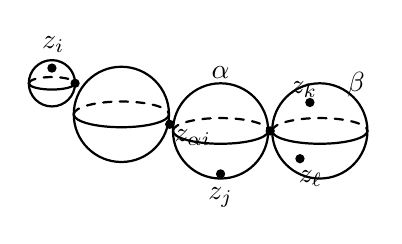
\begin{tikzpicture}[scale=.84,line width=.8pt,line cap=round]
  \newcommand{\Dfour}[3]{%
    \pgfmathsetmacro{\Dfleft}{#1-#3}%
    \pgfmathsetmacro{\Dfy}{.27*#3}%
    \draw (#1,#2) circle (#3);
    \draw[dashed] (\Dfleft,#2) arc[start angle=180,end angle=0,x radius=#3,y radius=\Dfy];
    \draw (\Dfleft,#2) arc[start angle=180,end angle=360,x radius=#3,y radius=\Dfy];}
  \Dfour{-2.2}{.25}{.72}
  \Dfour{-.7}{.0}{.72}
  \Dfour{.8}{.0}{.72}
  \Dfour{-3.25}{.72}{.35}
  \foreach \p in {(-2.9,.72),(-1.47,.1),(.05,.0),
    (-3.25,.95),(-.7,-.65),(.65,.43),(.5,-.42)}
    \fill \p circle (2pt);
  \node at (-3.23,1.30) {$z_i$};
  \node at (-1.12,-.1) {$z_{\alpha i}$};
  \node at (-.7,-1.0) {$z_j$};
  \node at (.56,.62) {$z_k$};
  \node at (.66,-.72) {$z_\ell$};
  \node at (-.7,.88) {$\alpha$};
  \node at (1.35,.7) {$\beta$};
\end{tikzpicture}

  \caption{边 $\alpha E\beta$ 的坐标 $w_{ijk\ell}$。}
  \label{fig:D-4-5}
\end{figure}

需证明：在给定点 $w^0\in\overline M_{0,n}$ 的邻域中，$w$ 的
所有分量都能表示成式~\eqref{eq:D-4-8} 和~\eqref{eq:D-4-9}
给出的 $n-3$ 个坐标的光滑函数。按边数归纳。先设
$T=\{\mathrm{pt}\}$，所选坐标即
$w_{1234},w_{1235},\ldots,w_{123n}$。
由 D.1 节的递推公式~\eqref{eq:D-1-3}，在开集
\[
  U:=\{w\in\overline M_{0,n}\mid
  w_{ijk\ell}\notin\{0,1,\infty\}\text{ 对所有 }i,j,k,\ell\},
\]
每个 $w_{ijk\ell}$ 都是 $w_{123m}$（$m=4,\ldots,n$）的光滑函数。
若 $i,j,k,\ell\in\{4,\ldots,n\}$，显式公式为
\[
  w_{ijk\ell}=
  \frac{(w_{123j}-w_{123k})(w_{123\ell}-w_{123i})}
  {(w_{123i}-w_{123j})(w_{123k}-w_{123\ell})}.
\]
此公式按 D.1 节式~\eqref{eq:D-1-2} 的规则扩展到任意
$i,j,k,\ell$：
\[
  w_{ijk\ell}=\begin{cases}
    \infty,&i=j\text{ 或 }k=\ell,\\
    1,&i=k\text{ 或 }j=\ell,\\
    0,&i=\ell\text{ 或 }j=k.
  \end{cases}
\]

现在设 $e(T)=\#\{\text{边}\}\ge1$，且边数严格较少的树已得结论。
任取边 $\alpha E\beta$。必要时重排指标，不妨设
\[
  I_{\beta\alpha}=\{1,\ldots,m\},\qquad
  I_{\alpha\beta}=\{m+1,\ldots,n\},\qquad
  i_{\beta\alpha}=m,\quad i_{\alpha\beta}=m+1,
\]
\sourcefootnote{原书在选边坐标时要求 $\alpha_n\in T_{\beta\alpha}$，
而此处又令 $I_{\beta\alpha}=\{1,\ldots,m\}$（$m<n$），从而
$n\notin I_{\beta\alpha}$。两处有向边的朝向约定不一致；
本段保留原记号，按此处两侧指标集合核对后续公式。}
且与边 $\alpha E\beta$ 对应的坐标为
\[
  y_{\alpha\beta}(w)=w_{1,m,m+1,n}.
\]
考虑投影 $w\mapsto w_I$ 与 $w\mapsto w_J$，其中
\[
  w_I:=\{w_{ijk\ell}\}_{i,j,k,\ell\le m+1},\qquad
  w_J:=\{w_{ijk\ell}\}_{i,j,k,\ell\ge m}.
\]
注意 $w_I^0\in\overline M_{0,m+1}$ 对应的树为 $T_{\beta\alpha}$；
其中第 $m+1$ 个\BookRecordIndex{T0066}标记点对应于 $w^0$ 中的边 $\alpha E\beta$。
按归纳假设，与 $T_{\beta\alpha}$ 的顶点和边相关的 $m-2$ 个坐标
均不含大于 $m+1$ 的指标，因而属于 $w_I$。
所以在 $w^0$ 的邻域中，凡 $i,j,k,\ell\in\{1,\ldots,m+1\}$，
$w_{ijk\ell}$ 都可由这些坐标光滑重建。
类似地，对 $i,j,k,\ell\in\{m,\ldots,n\}$，
所有分量都可由对应于 $T_{\alpha\beta}$ 的 $n-m-2$ 个坐标光滑重建。
剩下只需证明：在 $w^0$ 的某邻域中，$w$ 的所有分量
都可作为 $w_{1,m,m+1,n}$ 及所有满足
$i,j,k,\ell\le m$ 或 $i,j,k,\ell\ge m+1$ 的
$w_{ijk\ell}$ 的光滑函数。

为此先注意 $w_{1,m+1,n,m}(w^0)=0$。由
式~\eqref{eq:D-4-3}，对 $1<i<m$ 有
\[
  w_{m,m+1,n,i}=
  \frac{w_{1,m,m+1,i}-1}
  {w_{1,m,m+1,i}-w_{1,m,m+1,n}}.
\]
\sourcefootnote{原书印刷第637页此式的左端及分式有误。此处将
$(1,m,m+1,n,i)$ 代入式~\eqref{eq:D-4-3}，并据下文
$w_{m,m+1,n,i}(w^0)=0$ 补正。第二版作者勘误所列分式为
$(w_{1,m,m+1,n}-1)/(w_{1,m,m+1,n}-w_{1,m,m+1,i})$；
它在 $w_{1,m,m+1,n}(w^0)=\infty$ 时趋于 $1$ 而非 $0$，
故与此处递推式和紧接的论证仍不符。}
若取 $i\le m-1$，则 $w_{m,m+1,n,i}(w^0)=0$，由
式~\eqref{eq:D-4-3}，
\[
  w_{m+1,n,i,j}=
  \frac{w_{m,m+1,n,j}-1}
  {w_{m,m+1,n,j}-w_{m,m+1,n,i}}
\]
对所有 $j$ 成立。若再取 $i,j\le m$，则
$w_{m+1,i,j,n}(w^0)=0$，再用式~\eqref{eq:D-4-3}，
\[
  w_{i,j,k,n}=
  \frac{w_{m+1,i,j,n}-1}
  {w_{m+1,i,j,n}-w_{m+1,i,j,k}}
\]
对所有 $k$ 成立。最后，当 $\ell\ge m+1$ 时，
$w_{nij\ell}(w^0)=0$，故仍由式~\eqref{eq:D-4-3}，
\[
  w_{ijk\ell}=
  \frac{w_{nij\ell}-1}{w_{nij\ell}-w_{nijk}}
\]
对所有 $\ell\ge m+1$、$i,j\le m$ 及所有 $k$ 成立。
这样，在 $w^0$ 的某邻域中，只要 $i,j\le m$ 且
$k,\ell\ge m+1$，或者 $i,j,k\le m$ 且 $\ell\ge m+1$，
便已把 $w_{ijk\ell}$ 写成所需形式。
$i\le m$、$j,k,\ell\ge m+1$ 的情形由对偶性得到。
定理~\ref{thm:D-4-2} 得证。\qed

\begin{exercise}\label{ex:D-4-5}
上面在 $\overline{\mathcal M}_{0,n}$ 每个元素 $\mathbf z$ 附近构造了
显式坐标图。请用第 10 章采用的黏合与黏合参数语言来解释这些坐标图。
\end{exercise}

\noindent\textbf{分\BookRecordIndex{T0072}层。}
群 $G$ 作用于 $S^2$ 上 $n$ 个互异点组成的空间
$(S^2)^n\setminus\Delta_n$。商空间
\begin{equation}\label{eq:D-4-10}
  \mathcal M_{0,n}:=\frac{(S^2)^n\setminus\Delta_n}{G}
\end{equation}
是带 $n$ 个穿孔的二球面上复结构的\BookRecordIndex{T0246}模空间。此商空间不紧；
由嵌入 $\overline{\mathcal M}_{0,n}\to(S^2)^N$ 诱导拓扑的
$\overline{\mathcal M}_{0,n}$ 是它的
\emph{Grothendieck--Knudsen 紧化}。在
$\mathcal M_{0,n}\to\overline{\mathcal M}_{0,n}$ 的识别下，
子集 $\mathcal M_{0,n}$ 对应于
\begin{equation}\label{eq:D-4-11}
  M_{0,n}:=\{w\in\overline M_{0,n}\mid
  w_{ijk\ell}\notin\{0,1,\infty\}
  \text{ 对所有 }i,j,k,\ell\}.
\end{equation}
下一个命题说明，$\overline M_{0,n}$ 中\BookRecordIndex{T0106}顶层 $M_{0,n}$ 的补集
是有限个实余维为 $2$ 的光滑子流形之并。先引入记号。
给定 \BookRecordIndex{T0008}$n$-分割 $I\in\mathcal I_n$，令
\begin{equation}\label{eq:D-4-12}
  V_I:=\{w\in\overline M_{0,n}\mid I\in S(w)\}.
\end{equation}
因此，一条\BookRecordIndex{T0339}稳定曲线 $\mathbf z\in SC_{0,n}$ 满足
$w(\mathbf z)\in V_I$，当且仅当有一条边把 $I$ 中的\BookRecordIndex{T0066}标记点
与不在 $I$ 中的\BookRecordIndex{T0066}标记点分开。更一般地，对任意 \BookRecordIndex{T0008}$n$-分割网络
$S\in\mathcal S_n$，定义
\begin{equation}\label{eq:D-4-13}
  V_S:=\{w\in\overline M_{0,n}\mid S\subset S(w)\}
  =\bigcap_{I\in S}V_I.
\end{equation}
注意 $w(\mathbf z)\in V_S$ 当且仅当 $\mathbf z$ 的树结构是
$S$ 对应树结构的一个细化；还要注意 $V_\varnothing=\overline M_{0,n}$。

\begin{exercise}\label{ex:D-4-6}
令 $n=8$，且
$S=\bigl\{\{1,2\},\{3,4\},\{5,6\},\{1,2,3,4,5,6\}\bigr\}$。
描述 $V_S$ 中的元素，并验证下一个定理的 (iv)。
\end{exercise}

\begin{theorem}[Knudsen]\label{thm:D-4-7}
\begin{enumerate}
\item[(i)] 对每个 \BookRecordIndex{T0008}$n$-分割 $I\in\mathcal I_n$，子集
$V_I\subset\overline M_{0,n}$ 是复余维为 $1$ 的紧复子流形。
\item[(ii)] 若 $S\subset\mathcal I_n$，则
\[
  V_S\ne\varnothing\quad\Longleftrightarrow\quad S\in\mathcal S_n.
\]
\item[(iii)] 对每个 \BookRecordIndex{T0008}$n$-分割网络
$S=\{I_1,\ldots,I_m\}\in\mathcal S_n$，
子流形 $V_{I_1},\ldots,V_{I_m}$ 横截相交，因而
\[
  V_S=\bigcap_{j=1}^m V_{I_j}\subset\overline M_{0,n}
\]
是复余维 $\operatorname{codim}V_S=\#S$ 的复子流形。
\item[(iv)] 若 $S\in\mathcal S_n$ 对应\BookRecordIndex{T0084}带标号树 $(T,E,\Lambda)$，
且 $n_\alpha$ 由式~\eqref{eq:D-2-1} 对 $\alpha\in T$ 定义，
则存在微分同胚
\[
  V_S\cong\prod_{\alpha\in T}\overline M_{0,n_\alpha}.
\]
\end{enumerate}
\end{theorem}
\begin{proof}
断言 (i) 与 (iii) 直接由定理~\ref{thm:D-4-2}(iii) 证明中
坐标图的构造得出。为说明这一点，固定
$w^0=w(\mathbf z^0)\in\overline M_{0,n}$，
令 $I\in S(w^0)$ 为对应边 $\alpha E\beta$ 的 $w^0$-分割，
并设指标 $i,j,k,\ell$ 满足
\begin{equation}\label{eq:D-4-14}
  i,j\in I,\qquad k,\ell\notin I,\qquad
  z^0_{\alpha i}\ne z^0_{\alpha j},\qquad
  z^0_{\beta k}\ne z^0_{\beta\ell}.
\end{equation}
使用三项观察。首先，条件~\eqref{eq:D-4-14} 成立当且仅当
$I$ 是唯一把指标对 $\{i,j\}$ 与 $\{k,\ell\}$ 分开的
$w(\mathbf z^0)$-分割。其次，若 $w$ 充分接近 $w^0$，则
\[
  S(w)\subset S(w^0).
\]
第三，若 $w_{ijk\ell}=\infty$，则由引理~\ref{lem:D-4-4}(ii)
存在一个把 $\{i,j\}$ 与 $\{k,\ell\}$ 分开的 \BookRecordIndex{T0009}$w$-分割。
前两项观察说明这只能是 $I$。故当 $w$ 接近 $w^0$ 时，
\begin{equation}\label{eq:D-4-15}
  I\in S(w)\quad\Longleftrightarrow\quad w_{ijk\ell}=\infty.
\end{equation}
而定理~\ref{thm:D-4-2}(iii) 的证明表明，$w^0$ 附近有
$\overline M_{0,n}$ 的坐标图，其中每个 $w^0$-分割
$I\in S(w^0)$ 都由一个满足~\eqref{eq:D-4-14} 的坐标表示。
这证明 (i) 与 (iii)。

为证 (ii)，设 $S\subset\mathcal I_n$ 是不满足式~\eqref{eq:D-2-3}
的 \BookRecordIndex{T0008}$n$-分割集合。则存在 $I,J\in S$，使
\[
  I\cap J\ne\varnothing,\qquad I\setminus J\ne\varnothing,
  \qquad J\setminus I\ne\varnothing.
\]
此时引理~\ref{lem:D-4-3} 表明 $V_I\cap V_J=\varnothing$。

为证 (iv)，对每个 $\alpha\in T$ 取指标集
$I_\alpha\subset\{1,\ldots,n\}$，使其包含 $\Lambda_\alpha$，
并且对每条边 $\alpha E\beta$，恰好含有集合
$I_{\alpha\beta}(T,E,\Lambda)$ 的一个元素，
如定理~\ref{thm:D-4-2} 的证明。考虑只记住 $I_\alpha$ 中指标的投影
\[
  \pi_\alpha:\overline M_{0,n}\longrightarrow
  \overline M_{0,n_\alpha}.
\]
这些投影给出显然单射的映射
\[
  \pi_S:V_S\longrightarrow
  \prod_{\alpha\in T}\overline M_{0,n_\alpha}.
\]
为证其满射，任取元组 $\{w_\alpha\}_{\alpha\in T}$，
其中 $w_\alpha\in\overline M_{0,n_\alpha}$，并用树结构
重建其余分量 $w_{ijk\ell}$：若某 $I\in S$ 满足
$i,j\in I$、$k,\ell\notin I$，则定义 $w_{ijk\ell}=\infty$；
另外两种配对分割的情形同理。若不存在把四指标分成两对的分割，
则存在顶点 $\alpha$ 与四个互异指标
  $i',j',k',\ell'\in I_\alpha$，使 $i=i'$ 或
$\alpha_i,\alpha_{i'}\in T_{\alpha\beta}$\sourcefootnote{原书此处写 $i,i'\in T_{\alpha\beta}$；$i,i'$ 是指标，而 $T_{\alpha\beta}$ 是顶点集。依本节 $I_{\alpha\beta}$ 的定义，改作指标所标记的顶点属于该分支。} 对某条边 $\alpha E\beta$ 成立；
$j',k',\ell'$ 亦然。在这种情形令
$w_{ijk\ell}:=w_{i'j'k'\ell'}$。
容易验证这样定义的元组 $w$ 满足式~\eqref{eq:D-4-2}
与~\eqref{eq:D-4-3}，因而属于 $\overline M_{0,n}$。
这说明 $\pi_S$ 是满射，且其逆映射光滑，定理得证。
\end{proof}
